\chapter{Introduction}
\label{ch_intro}


Since the discovery of the $\jpsi$ particle in 1974, the charm energy range (\SIrange{3.0}{4.5}{\GeV}) has been one of the most precisely studied regions in particle physics.
This has led to the further discovery of many more resonances, as shown in \Cref{fig:R_scan}.

\begin{figure}[H]
\centering
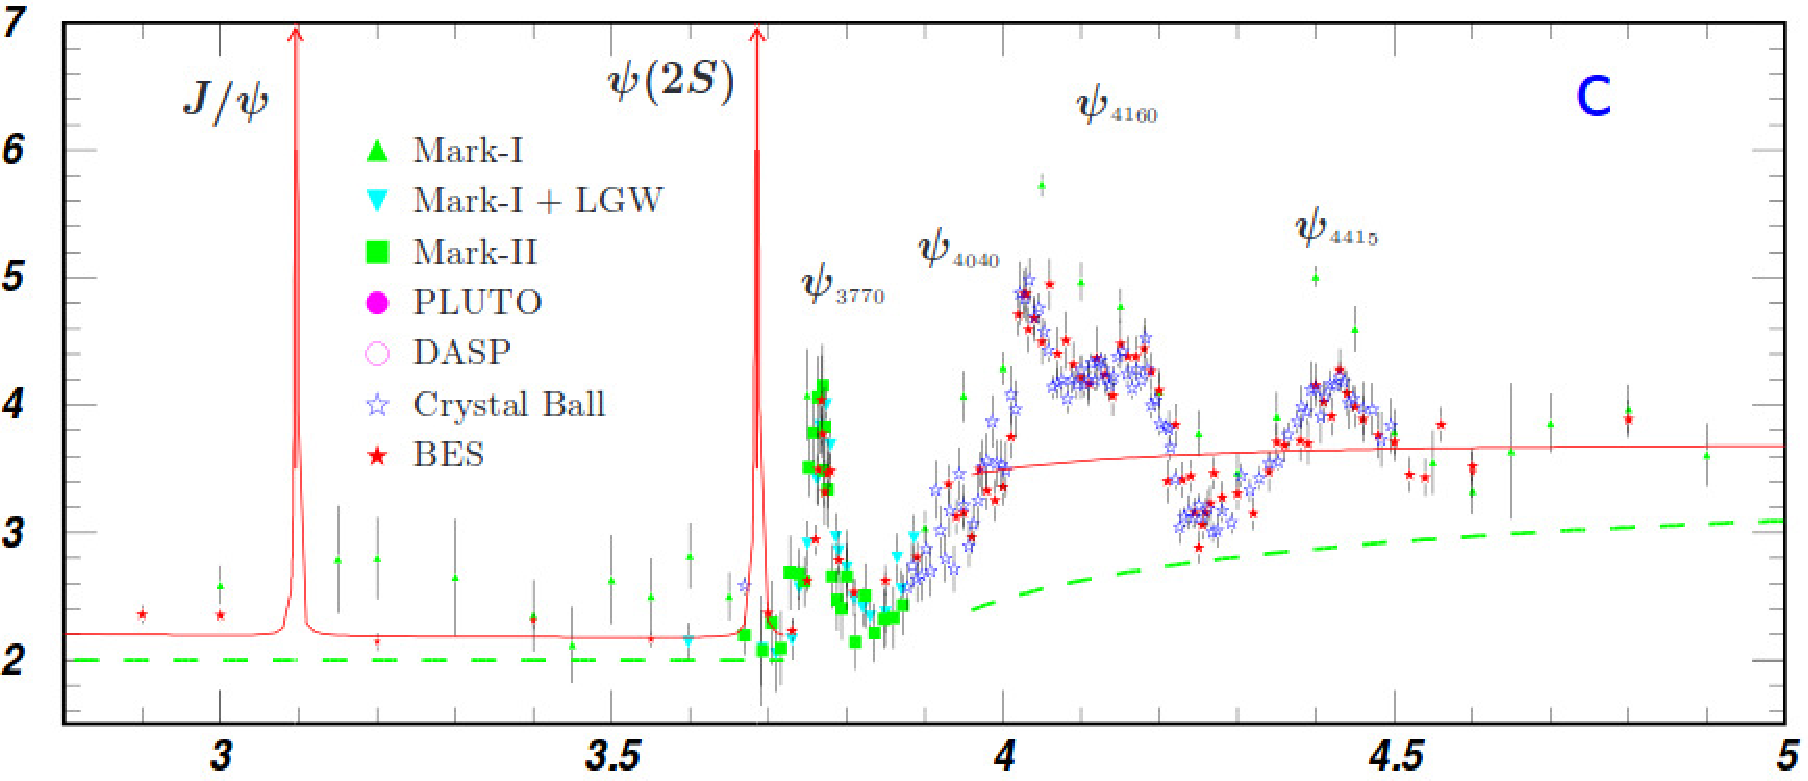
\includegraphics[scale=0.50]{figures/images/R_scan.pdf}
\caption{Measurements of $R = \sigma(\ee \rightarrow \text{hadrons}) / \sigma(\ee \rightarrow \mumu)$.}
\label{fig:R_scan}
\end{figure}

Many of the lower mass resonances are predictable within the context of the quark model.
However, there are a number of states which have been predicted, but not yet discovered.
There are also states which were discovered experimentally without any corresponding predictions.
A variety of these particles are shown in \Cref{fig:charmonia}.

\begin{figure}[H]
\centering
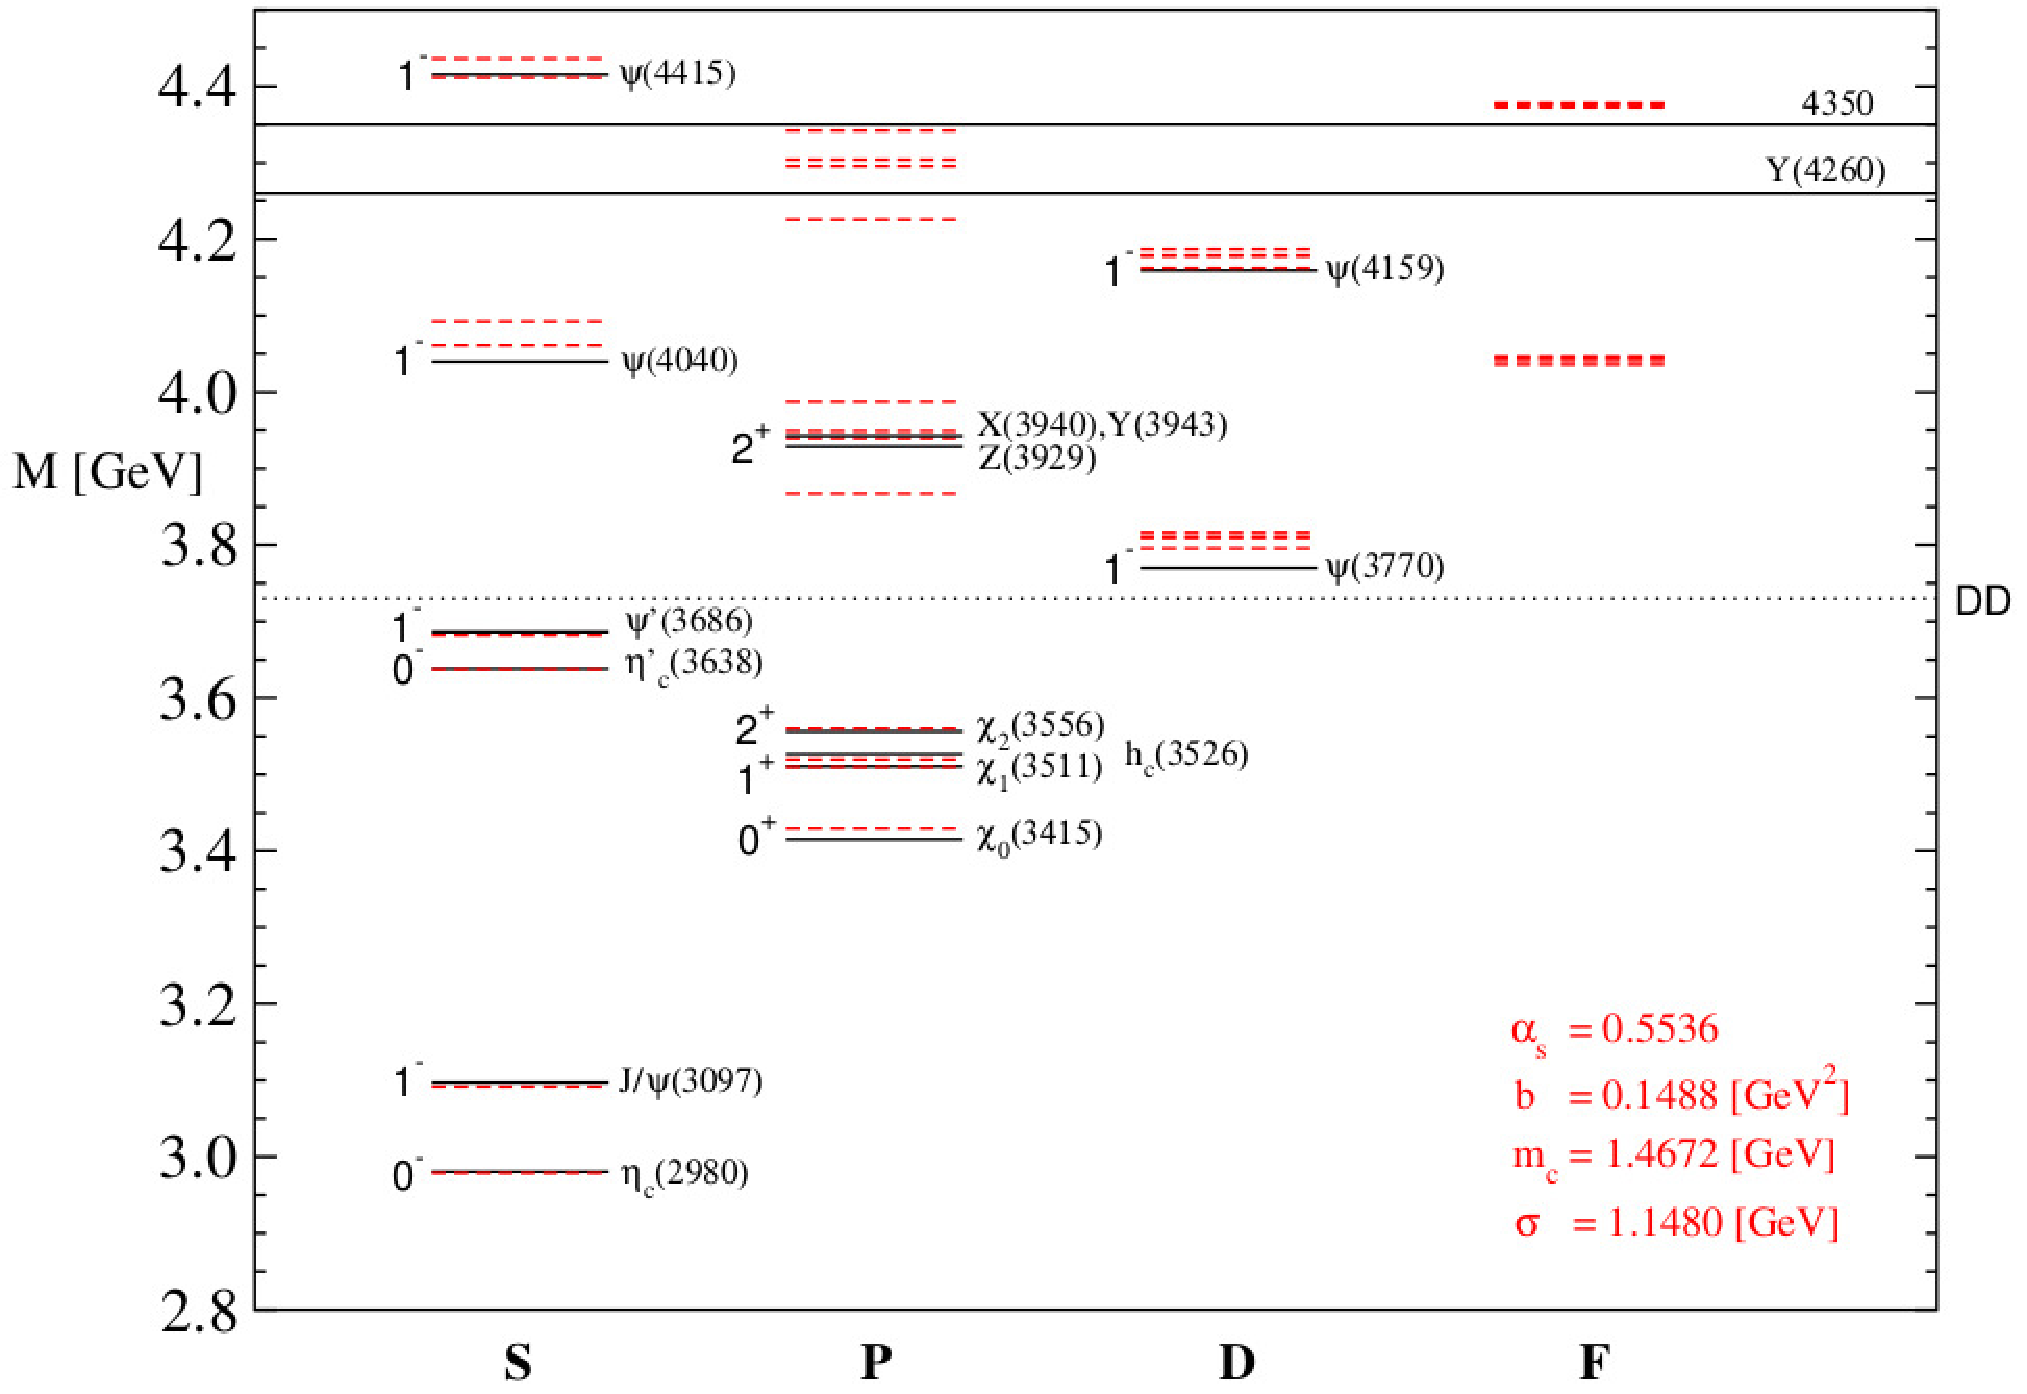
\includegraphics[scale=0.40]{figures/images/charmonia.pdf}
\caption{Measured and predicted charmonium resonances.}
{Solid black lines represent measurements while the dashed red lines are predictions.}
\label{fig:charmonia}
\end{figure}

The resonances below the $\DDbar$ threshold, like the $\jpsi$ and the $\psip$, show solid agreement with their theoretical predictions.
However, many of the ones above, such as the $\psipp$, still show some disagreement.
This is likely due to the more complicated interactions introduced from $\DDbar$ decays.
Several experiments have attempted to measure the shape of the $\psipp$ based on different assumptions.
The most prominent of these is the assumption of interference.
This can have notable effects on the resultant parameters of the $\psipp$, such as the mass, shown in \Cref{tab:previous_results}.

\begin{table}[H]
\centering
\begin{tabular}{c l|c l}
\hline
\multicolumn{2}{c|}{$\Mpsipp$ [\si{\MeV}] (No Interference)} & \multicolumn{2}{c}{$\Mpsipp$ [\si{\MeV}] (With Interference)} \\ [1pt] 
\hline
BES-II \cite{ref:Ablikim:2007}   & 3772.0 $\pm$ 1.9           & BaBar \cite{ref:Aubert:2008b} & 3778.8 $\pm$ 1.9 $\pm$ 0.9 \\
Belle  \cite{ref:Brodzicka:2008} & 3776.0 $\pm$ 5.0 $\pm$ 4.0 & KEDR  \cite{ref:Anashin:2012} & $3779.2^{+1.8 \, +0.5 \, +0.3}_{-1.7 \, -0.7 \, -0.3}$ \\ 
BaBar  \cite{ref:Aubert:2008a}   & 3775.5 $\pm$ 2.4 $\pm$ 0.5 & & \\
\hline
\end{tabular}
\caption{Previous experimental results for the mass of the $\psipp$.}
{Where applicable, the first errors are statistical, the second are systematic, and the third are model-dependent.}
\label{tab:previous_results}
\end{table}

Both BaBar \cite{ref:Aubert:2008b} and KEDR \cite{ref:Anashin:2012} found it necessary to include interference effects for fitting the $\DDbar$ spectrum.
However, the statistics of the KEDR sample were insufficient to fully resolve the discrepancies seen with other experiments that ignored interference.
{\bf Using the larger data sample available at BESIII, we have precisely measured and analyzed the shape of the $\DDbar$ spectrum around the $\psipp$ resonance.}
We have also used this measurement to probe the branching fraction of $\nonDDbar$ decays in this region.


\section{Procedure}
\label{sec:procedure}

The basis of this measurement involves identifying $\DDbar$ pairs which have decayed from $\psipp$.
All data used in this analysis was collected from $\ee$ collisions analyzed by the BESIII detector.
As $\lel$ and $\alel$ are fundamental particles, the total energy of each is transferred in the collision.
Additionally, the ability to precisely tune these two beam energies allows for the targeted production of specific particles, such as the $\psipp$.
However, resonances like this will decay almost instantaneously.
For example, the $\psipp$ has an average lifetime of ${\sim}\SI{e-23}{\s}$.
Even if it were traveling at $c$, the farthest distance this could travel would be $(\SI{3e8}{m/s}) \times ({\sim}\SI{e-23}{\s}) \approx \SI{1}{\fm}$.
This distance, approximately the radius of a proton, is far too small to be resolved by our detectors.
Even the initial decay into $\DDbar$ pairs is too small to precisely measure, as their lifetime of \SI{~4e-13}{\s} corresponds to a maximum distance of ${\sim}\SI{1}{\mm}$ if it were traveling at $c$.
However, the limited available energy in these decays ($m_{\psipp} - 2 \times m_{D} \approx \SI{40}{\MeV})$ means the velocity is much, much slower.

% \tau = 1 / 25 [1/MeV] * (200 MeV / 1e-15 m) / (3e8 m / s) = 200 / (3 * 25) e-23 s ~ 10^-13 s

Instead, the reconstruction of candidate $D$ particles relies on measuring their decays into other known modes.
While there are dozens of possible decays modes, we focus on those which have high branching fractions, and are comprised of particles identifiable by the BESIII detector.
For our purposes, these are $\pipm, \Kpm, \piO,$ and $\Ks$.
Each of these particles leave `tracks' within the detector; charged particles travel along curved paths and interact electromagnetically with charged wires along their trajectory, while neutral particles travel along straight paths and deposit bursts of energy after contacting crystals located along the inner walls of the detector.
The various components of the BESIII detector analyze these tracks to determine the type of particle, as well as its momentum and energy.
By analyzing sets of particles corresponding to the chosen decay modes, we can reconstruct the combination most likely to have originated from a $D$ based on their total energy.


To determine the $\psipptoDD$ cross section, we need to count the number of $\DDbar$ pairs produced, as well as measure the integrated luminosity, at each energy point in our data sample.
This counting is done not only for the actual collision data collected, but also for computed generated Monte Carlo (MC) background samples.
Each of these backgrounds corresponds to a particular event type which may be mistaken as signal, such as $\ee \rightarrow \tautau$.
We subtract these misidentified contributions from the total amount found in data to determine the actual number of reconstructed $\DDbar$ events.
Also from MC, we calculate the efficiency of reconstructing $\DDbar$ decays based on our selection criteria.
By dividing the actual reconstructed events by this efficiency, we identify the true number of $\DDbar$ events produced.
Then, using the measured luminosity for each energy point, we determine the cross section as a function of center-of-mass energy.

% 
% While energy and momentum conservation remain fundamental laws of physics, accounting for the 
% 
% Also must correct for initial state radiation
% Accelerated particles (such as those traveling around a circular collider) radiate energy
% This energy reduces the total amount available in a collision
% Can lead to producing lower resonances (jpsi, psip) instead of targeted psipp
% Also decreases total energy available at each point, and must be accounted for
% Effect is very calculable, and included in cross section derivation


The specific details of this analysis start with background on relevant theoretical concepts.
Next, we list the specifications for the collider and detector which collected the data used for these measurements along with their related analysis software and reconstruction methods. 
From here, we further describe the procedure for determining the $\psipptoDD$ cross section and show the results with systematic uncertainties.
Finally, we examine the current progress of measuring the $\nonDDbar$ branching fraction.

